
\documentclass[a4paper,12pt]{article}

\usepackage{graphicx} % Required for inserting images
\usepackage{amsmath,amssymb,amsfonts}
\usepackage{subcaption}
% -----------------------
% Package Imports
% -----------------------

% Set page margins
\usepackage[a4paper, top=1in, bottom=0.8in, left=1.1in, right=0.8in]{geometry}

% Use Times New Roman font
\usepackage{times}

% Add page numbering
\pagestyle{plain}

% Enable graphics inclusion
\usepackage{graphicx}
\usepackage{float}
% Enable code listings
\usepackage{listings}
\usepackage{xcolor} % For customizing code colors
\setlength{\parindent}{0pt}
\usepackage{physics}
\usepackage{multirow}


\begin{document}
	\section{Experiment No. 10}
	
	\section{Experiment Title }
Three-Phase Transformer using Two Single-Phase Transformers (Open-$\Delta-\Delta$ Connection)
	\section{Objective}
	
	The objectives of this lab are as follows:

\begin{itemize}
	\item To analyze the performance of a three-phase transformer using an open-$\Delta$ connection.
	\item To calculate and compare the power delivered in the closed-$\Delta$ and open-$\Delta$ configurations.
	\item To determine the power ratio and validate the theoretical reduction in power capacity.
	\item To understand the effects of using an open-$\Delta$ connection in terms of power factor and load capacity.
\end{itemize}
	\section{Theory}
	
	\subsection{Open-Delta (V-V) Connection}
	
	The open-delta or V-V connection is a method of transforming three-phase power using only two transformers instead of three. It is utilized in the following cases:
	\begin{enumerate}
		\item When the three-phase load is too small to justify the installation of a full three-phase transformer bank.
		\item When one transformer in a $\Delta-\Delta$ bank fails, enabling service continuity at reduced capacity.
		\item When there is a future expectation of increased load, allowing for the open-delta to be closed later to form a $\Delta-\Delta$ bank.
	\end{enumerate}
	
	In a V-V connection, the transformer bank's capacity is reduced compared to the $\Delta-\Delta$ configuration. The ratio of V-V capacity to $\Delta-\Delta$ capacity can be derived as follows:
		\subsection{Derivation of Capacity Ratio}
	
	For a $\Delta-\Delta$ transformer bank, the total capacity is:
	\[
	P_{\Delta-\Delta} = \sqrt{3} \, V_L \, I_L,
	\]
	where \( V_L \) is the line voltage, and \( I_L \) is the line current.
		In the case of a V-V connection, the capacity is:
	\[
	P_{\text{V-V}} = 2 \cdot (\text{per-transformer capacity}).
	\]
	\begin{figure}[H]
		\centering
		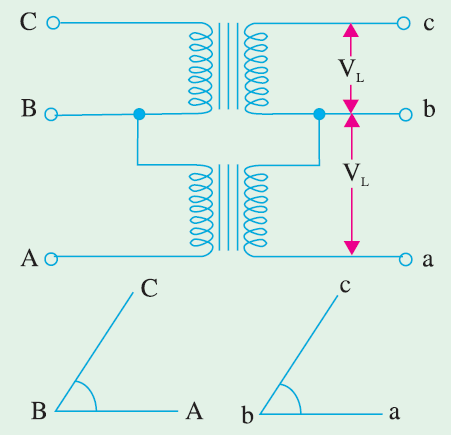
\includegraphics[width=0.5\linewidth]{screenshot001}
		\caption{Open-Delta (V-V) Connection}
		\label{fig:screenshot001}
	\end{figure}

	

	Here, the line current in a V-V connection equals the phase current \( I_S \), so:
	\[
	P_{\text{V-V}} = \sqrt{3} \, V_L \, I_S,
	\]
	and \( I_S = I_L / \sqrt{3} \). Substituting this relationship gives:
	\[
	P_{\text{V-V}} = \sqrt{3} \, V_L \, \left(\frac{I_L}{\sqrt{3}}\right) = V_L \, I_L.
	\]
	
	The ratio of V-V capacity to $\Delta-\Delta$ capacity is then:
	\[
	\text{Capacity Ratio} = \frac{P_{\text{V-V}}}{P_{\Delta-\Delta}} = \frac{V_L \, I_L}{\sqrt{3} \, V_L \, I_L} = \frac{1}{\sqrt{3}} \approx 0.577.
	\]
	
	This demonstrates that the V-V connection's capacity is approximately \( 57.7\% \) of the full $\Delta-\Delta$ capacity.
	
	\subsection{Key Properties of V-V Connection}
	
	1. \textbf{Utility Factor:} The available capacity of a V-V bank is \( 86.6\% \) of the combined ratings of the two transformers:
	\[
	\text{Utility Factor} = \sqrt{3}/2 \approx 0.866.
	\]
	
	2. \textbf{Load per Transformer:} Each transformer carries \( 57.7\% \) of the total load:
	\[
	\text{Load per Transformer} = \frac{\text{Total Load}}{2} \times \frac{1}{\sqrt{3}}.
	\]
	
	3. \textbf{Overload in Open-Delta Operation:} If one transformer is removed from a fully-loaded $\Delta-\Delta$ bank, the remaining transformers experience overload:
	\[
	\text{Overload Factor} = \sqrt{3} \approx 1.732 \, (\text{or } 73.2\%).
	\]
	
	\subsection{Disadvantages of V-V Connection}
	
	1. The average power factor of the V-V bank is lower than the load power factor:
	\[
	\text{Power Factor of V-V Bank} = 0.866 \times \text{Load Power Factor}.
	\]
	
	2. The secondary terminal voltages become unbalanced as the load increases, even for a balanced load.
	
	\subsection{Power Supplied by V--V Bank}
	
	When a V--V bank of two transformers supplies a balanced 3-phase load of power factor $\cos \phi$, then one transformer operates at a power factor of $\cos (30^\circ - \phi)$ and the other at $\cos (30^\circ + \phi)$. Consequently, the two transformers will not have the same voltage regulation.
	
	\[
	P_1 = \text{kVA} \cos (30^\circ - \phi) \quad \text{and} \quad P_2 = \text{kVA} \cos (30^\circ + \phi)
	\]
	
	\subsection*{Case 1: When $\phi = 0$ (i.e., load p.f. = 1)}
	Each transformer will have a power factor:
	\[
	\cos 30^\circ = 0.866
	\]
	
	\subsection*{Case 2: When $\phi = 30^\circ$ (i.e., load p.f. = 0.866)}
	In this case, one transformer has a power factor:
	\[
	\cos (30^\circ - 30^\circ) = 1
	\]
	and the other has a power factor:
	\[
	\cos (30^\circ + 30^\circ) = 0.866
	\]
	
	\subsection*{Case 3: When $\phi = 60^\circ$ (i.e., load p.f. = 0.5)}
	In this case, one transformer will have a power factor:
	\[
	\cos (30^\circ - 60^\circ) = \cos (-30^\circ) = 0.866
	\]
	and the other will have a power factor:
	\[
	\cos (30^\circ + 60^\circ) = 0
	\]
	It means that one of the transformers will not supply any load, whereas the other having a power factor of $0.866$ will supply the entire load.
	


	
	\newpage
	\section{Required Apparatus}
	\begin{enumerate}
		\item \textbf{Transformer}
		\begin{enumerate}
			\item Power (\(P\)): 760 VA
			\item Primary Voltage (\(U_1\)): 230 V
			\item Secondary Voltage (\(U_2\)): 400 -- 230 V
			\item Frequency (\(f\)): 50 Hz
			\item Primary Current (\(i_1\)): 3.7 A
			\item Secondary Current (\(i_2\)): 1 -- 1.7 A
		\end{enumerate}
		\item \textbf{Voltmeter:} 500 V AC rms MAX
		\item \textbf{Ammeter:} 5 A MAX
		\item \textbf{Digital Multimeter Display}
		\item \textbf{Connecting Wires}
		\item \textbf{Variable Three Phase AC Line:} 
		\begin{enumerate}
			\item \textbf{Voltage:} 430V
			\item \textbf{Current:} 3A
		\end{enumerate}
		\item \textbf{Variable Resistor:} 
		\begin{enumerate}
			\item \textbf{Resistance:} $3 \times 50 \, \Omega$
			\item \textbf{Current:} $3 \times 3.16 \, \mathrm{A}$
		\end{enumerate}
			\end{enumerate}


	\section{Circuit Diagrram}
	
	
	\begin{figure}[H]
	
	
			\centering
			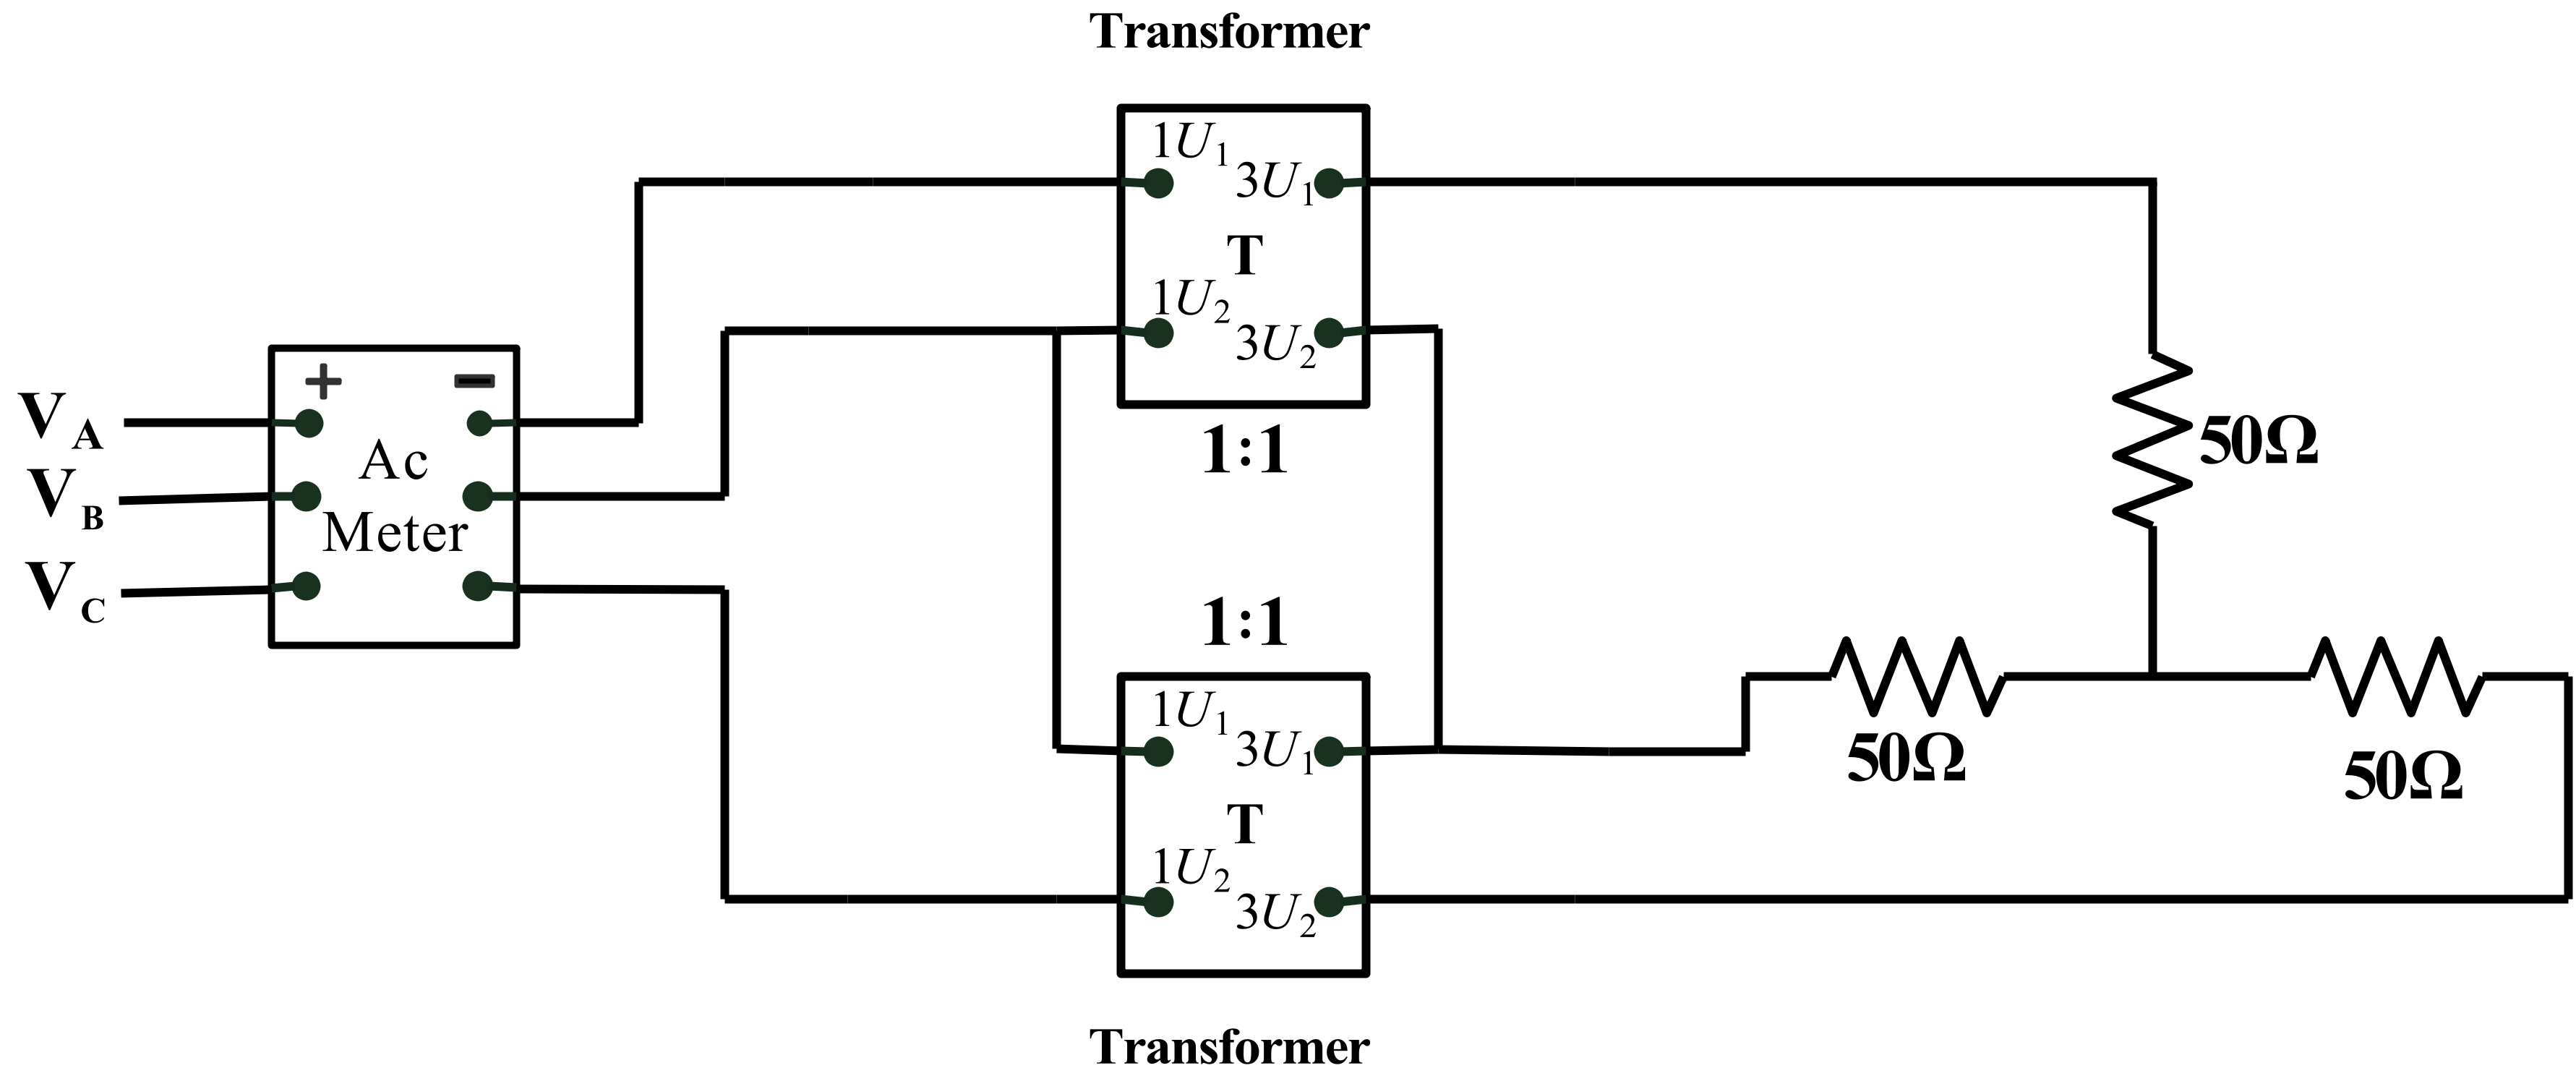
\includegraphics[width=1\linewidth]{Images/exp10}
			\caption{Connection for Three-Phase Transformer using Two Single-Phase.}
		
		
	\end{figure}
	
	
	\newpage
	
	
	\section{Data Table}
\begin{table}[h!]
	\centering
	\begin{tabular}{|c|c|c|c|c|c|c|c|}
		\hline
		\begin{tabular}[c]{@{}c@{}}$V_{A}$\\ (V)\end{tabular} & \begin{tabular}[c]{@{}c@{}} $V_{B}$ \\ (V)\end{tabular} & \begin{tabular}[c]{@{}c@{}}$V_{C}$\\ (V)\end{tabular} & \begin{tabular}[c]{@{}c@{}}$I_a$\\ (A)\end{tabular} & \begin{tabular}[c]{@{}c@{}}$I_b$\\ (A)\end{tabular} & \begin{tabular}[c]{@{}c@{}}$I_c$\\ (A)\end{tabular} & \begin{tabular}[c]{@{}c@{}}$P_{\text{open}}$\\ (W)\end{tabular} & \begin{tabular}[c]{@{}c@{}}$P_{\text{close}}$\\ (W)\end{tabular} \\ \hline
		\multirow{3}{*}{165.1}                                & \multirow{3}{*}{163.1}                                   & \multirow{3}{*}{157.7}                                & \multirow{3}{*}{1.69}                               & \multirow{3}{*}{1.73}                               & \multirow{3}{*}{1.67}                               & 106.0                                                               & \multirow{3}{*}{824.541}                                          \\ \cline{7-7}
		&                                                          &                                                       &                                                     &                                                     &                                                     & 267.2                                                               &                                                                   \\ \cline{7-7}
		&                                                          &                                                       &                                                     &                                                     &                                                     & 110.0                                                               &                                                                   \\ \hline
	\end{tabular}
	\caption{Measured Values and Power for Three-Phase System}
	\label{tab:three_phase_system}
\end{table}
\section{Calculations}

Using the measured data in Table~\ref{tab:three_phase_system}, the following calculations are performed:

\begin{enumerate}
	\item \textbf{Closed-Circuit Power, $P_{\text{closed}}$:}  
	The total closed-circuit power is calculated as:
	\[
	P_{\text{closed}} = V_{A} \cdot I_a + V_{B} \cdot I_b + V_{C} \cdot I_c
	\]
	Substituting the values from the table:
	\[
	P_{\text{closed}} = (165.1 \cdot 1.69) + (163.1 \cdot 1.73) + (157.7 \cdot 1.67)
	\]
	Performing the calculations:
	\[
	P_{\text{closed}} = 279.019 + 282.163 + 263.359 = 824.541 \, \text{W}
	\]
	
	\item \textbf{Open-Circuit Power, $P_{\text{open}}$:}  
	The open-circuit power is the sum of the individual measurements:
	\[
	P_{\text{open}} = (106.0 + 267.2 + 110.0) \, \text{W}
	\]
	Adding the values:
	\[
	P_{\text{open}} = 483.2 \, \text{W}
	\]
	
	\item \textbf{Required Ratio:}  
	The ratio of open-circuit power to closed-circuit power, expressed as a percentage, is calculated as:
	\[
	\text{Required Ratio} = \left( \frac{P_{\text{open}}}{P_{\text{closed}}} \right) \times 100\%
	\]
	Substituting the values:
	\[
	\text{Required Ratio} = \left( \frac{483.2}{824.541} \right) \times 100\%
	\]
	Performing the division:
	\[
	\text{Required Ratio} \approx 58.6\%
	\]
\end{enumerate}

	\newpage
\section{Discussion}

The experiment was successfully conducted to analyze the performance of a three-phase transformer using two single-phase transformers in an open-$\Delta$ connection. It was found that the power delivered in the open-$\Delta$ configuration was approximately 58.6\% of the power delivered in the closed-$\Delta$ configuration. This reduction in power was consistent with theoretical expectations, where the power delivered in an open-$\Delta$ system is approximately 57.7\%.

The measured closed-circuit power was found to be \( P_{\text{closed}} = 824.541 \, \text{W} \), and the open-circuit power was \( P_{\text{open}} = 483.2 \, \text{W} \), resulting in a power ratio of \( \approx 58.6\% \). This confirmed the theoretical reduction in capacity when one transformer was removed from the system.

It was concluded that the open-$\Delta$ connection can be used to continue service at reduced capacity, but with a significant drop in power delivery compared to the full closed-$\Delta$ system. The variation in power factor across the transformers highlighted the importance of careful load management in such configurations.

\end{document}
